\documentclass[10pt, conference]{IEEEtran}
\IEEEoverridecommandlockouts
\usepackage{cite}
\usepackage{amsmath,amssymb,amsfonts}
\usepackage{graphicx}
\usepackage{textcomp}
\usepackage{xcolor}
\usepackage{booktabs}
\usepackage{multirow}
\usepackage{threeparttable}
\usepackage{xfp}

\DeclareMathOperator*{\argmax}{argmax}
\DeclareMathOperator*{\argmin}{argmin}
\newcommand{\etal}{\textit{et al. }}
\newcommand{\red}[1]{\textcolor{red}{#1}}
\newcommand{\blue}[1]{\textcolor{blue}{#1}}


\def\BibTeX{{\rm B\kern-.05em{\sc i\kern-.025em b}\kern-.08em
    T\kern-.1667em\lower.7ex\hbox{E}\kern-.125emX}}
\begin{document}

\title{Lightweight RF Fingerprinting via PCA-Driven Channel Pruning and Self-Distillation}

\author{
\IEEEauthorblockN{
Keyi~Mo\IEEEauthorrefmark{1},
Guanxiong~Shen\IEEEauthorrefmark{1}\IEEEauthorrefmark{2}
}

\IEEEauthorblockA{
\IEEEauthorrefmark{1}
School of Cyber Science and Engineering, Southeast University, Nanjing, China
}
\IEEEauthorblockA{
\IEEEauthorrefmark{2}
Corresponding Author
}

}

\maketitle


\begin{abstract}
Radio frequency fingerprint identification (RFFI) is a physical-layer authentication technique that identifies wireless devices through hardware-inherent imperfections. Recent deep learning-based RFFI systems achieve high accuracy but cannot support real-time, per-packet inference on resource-constrained edge devices. Existing lightweight solutions rely on hand-crafted architectures or heuristic pruning, whose compression ratios follow human intuition rather than learned representations. This paper presents an automated lightweight RFFI pipeline that exploits principal component analysis (PCA) in two complementary roles. First, PCA-driven channel pruning analyzes feature maps to automatically determine each layer's effective dimension that preserves 95\% cumulative variance, eliminating hand-picked compression ratios. Second, PCA-aligned distillation projects the teacher's high-dimensional embedding space into the student's low-dimensional space, enabling effective knowledge transfer despite dimensional mismatch. The compact student is randomly initialized and trained via temperature-scaled KL divergence in the shared subspace. An optional iterative mode enables accuracy-bounded progressive compression. Experiments on four architectures with a real-world LoRa dataset demonstrate 14--834$\times$ parameter compression with minimal accuracy loss and sub-millisecond inference on NVIDIA Jetson platforms. The distilled student can even outperform an undertrained teacher.
\end{abstract}


\begin{IEEEkeywords}
Physical layer security, radio frequency fingerprinting, model compression, principal component analysis, knowledge distillation.
\end{IEEEkeywords}


\section{Introduction}

Radio frequency fingerprint identification (RFFI) is a physical-layer authentication technique that identifies wireless devices through their hardware-inherent imperfections. Analog components in the transmitter chain, such as oscillators, mixers, and power amplifiers, inevitably deviate from their nominal specifications during manufacturing. These deviations imprint unique distortions on the emitted signal, which are difficult to clone or forge and therefore serve as device identifiers. RFFI is particularly attractive for Internet of Things (IoT) systems, where resource-constrained devices cannot afford conventional cryptographic authentication. State-of-the-art RFFI methods leverage deep learning, such as convolutional neural networks (CNNs) operating on spectrograms or raw I/Q samples, and achieve high identification accuracy with strong robustness to channel variations~\cite{9488793,9715147}.

Practical RFFI deployment, however, imposes stringent real-time requirements. RFFI verification operates on a per-packet basis: every received packet must be authenticated before delivery to upper layers, so that illegitimate packets can be rejected immediately. The inference latency therefore directly adds to packet processing delay, and slow verification can stall the reception pipeline. Modern RFFI systems require sub-millisecond inference on edge platforms to support real-time per-packet authentication. This requirement conflicts with the high-capacity architectures behind accurate RFFI, such as deep convolutional and residual networks~\cite{7780459}. These over-parameterized models exceed the latency and energy budgets of edge hardware. Structural model compression is therefore essential for practical RFFI deployment.

\textbf{Limitations of existing lightweight RFFI approaches.}
[PLACEHOLDER: This paragraph will review existing lightweight RFFI methods and their limitations. Future work will add 3-5 references covering: (1) manually designed compact RFFI architectures, (2) uniform pruning methods applied to RFFI, (3) other compression techniques for RFFI. The paragraph should emphasize that existing approaches rely on manual design or uniform compression ratios that do not account for layer-wise heterogeneity in learned RF representations.]

General-purpose lightweight neural network design has been extensively studied. One approach redesigns the architecture for efficiency: MobileNets~\cite{howard2017mobilenetsefficientconvolutionalneural}, for example, replace standard convolutions with depthwise separable convolutions and apply a uniform width multiplier. Another approach compresses trained networks through channel pruning based on hand-picked importance criteria. While these paradigms have been applied to RFFI, they share a fundamental limitation: compression ratios are dictated by manual intuition rather than the intrinsic characteristics of learned representations. A uniform width multiplier assumes homogeneous redundancy across all layers, which does not hold in RFFI networks. Physical-layer signal features exhibit strong layer-wise heterogeneity: shallow layers encode low-level time-frequency textures while deep layers capture abstract device-specific patterns. Uniform compression therefore damages information-critical layers while leaving redundant layers unnecessarily wide.

\textbf{Our approach.}
A key observation underpins this work: a fully trained high-capacity network inherently encodes its own architectural redundancy. The channel-wise energy spectrum obtained by principal component analysis (PCA) on feature maps analytically reveals the exact dimension required to retain the dominant representation variance at each layer. We propose an automated lightweight RFFI framework that exploits PCA in two complementary roles. First, PCA-driven channel pruning automatically determines per-layer compression ratios from feature variance. Second, PCA-aligned distillation bridges the dimensional gap between teacher and student embedding spaces by projecting the teacher's high-dimensional embeddings into the student's low-dimensional space. An optional iterative mode repeats this pipeline under a configurable accuracy floor, enabling progressive compression without manual tuning.

We evaluate the framework on four diverse architectures with a real-world LoRa dataset and demonstrate sub-millisecond inference on NVIDIA Jetson edge platforms. The main contributions are:
\begin{itemize}
    \item We propose a PCA-driven channel pruning method that analyzes the feature variance of each convolutional layer to automatically derive its effective dimension, eliminating hand-picked compression ratios. It achieves 14--834$\times$ parameter compression across four architectures with minimal accuracy loss, and the resulting students run in as little as 0.69~ms on an NVIDIA Jetson Nano.

    \item We design a PCA-aligned distillation paradigm that projects the teacher's high-dimensional embedding space into the student's low-dimensional space, enabling effective knowledge transfer despite dimensional mismatch. The distilled student can outperform an undertrained teacher: the 834$\times$-compressed DenseNet student achieves higher accuracy than its teacher on 11 of 12 test scenarios.

    \item We develop an iterative compression mode that progressively applies PCA-driven pruning and aligned distillation under a configurable accuracy bound. It reaches 67.2$\times$ cumulative compression on ResNet after two rounds, with accuracy improved after the first round.
\end{itemize}

\section{System Overview}

\begin{figure}[t]
    \centering
    \includegraphics[width=0.95\linewidth]{figures/Overview of an RF Fingerprinting System.pdf}
    \caption{System architecture of the proposed automated lightweight RFFI framework. The compression pipeline employs PCA in two complementary roles: PCA-driven channel pruning determines the student architecture, and PCA-aligned distillation trains the student parameters (Section~III).}
    \label{fig:system_arch}
\end{figure}

Fig.~\ref{fig:system_arch} illustrates the overall workflow of the proposed framework, which operates in three stages: model compression, device enrollment, and runtime authentication. The model compression stage applies two PCA-based techniques iteratively: PCA-driven channel pruning analyzes the teacher's convolutional feature maps to determine the effective channel count per layer, and PCA-aligned distillation trains the pruned student by projecting the teacher's embedding space into the student's lower-dimensional space. The trained student then becomes the teacher for the next iteration. This loop continues until the accuracy degradation exceeds a predefined threshold $\delta$. Section~III presents the algorithmic details.

\subsection{Model Compression Pipeline}

The compression pipeline consists of three modules that exploit PCA in complementary roles.
\begin{itemize}
    \item \textbf{Teacher Network Training} (Section~III-A) produces a high-capacity teacher that establishes a discriminative embedding space. The trained teacher serves two roles: its convolutional feature maps provide the input for PCA-driven channel analysis, and its embeddings serve as soft supervision targets for distillation.
    \item \textbf{Single-Round Compression} (Section~III-B) combines PCA-driven channel pruning and PCA-aligned distillation into one compression cycle. Channel pruning analyzes feature variance to determine the student architecture, and distillation trains the randomly initialized student via embedding space alignment.
    \item \textbf{Iterative Compression} (Section~III-C) extends the single-round procedure to a multi-round loop under an accuracy-bounded schedule. The student from round $r$ becomes the teacher for round $r+1$, enabling progressive compression until the accuracy floor $\delta$ is reached.
\end{itemize}
This pipeline is executed once by a model provider with sufficient computational resources and does not impose real-time constraints.

\subsection{Device Enrollment and Authentication}

After the compression pipeline completes, the resulting compact student network is deployed to edge devices for authentication. During enrollment, a small number of packets are collected from each authorized device under controlled conditions. The student network extracts embeddings from these packets, which are stored as reference templates in a local database. During authentication, each received packet is authenticated in real time: the student extracts its embedding and compares it against the enrolled templates via $k$-nearest neighbor (KNN) search with Euclidean distance. The packet is accepted if it matches a known device or rejected otherwise. Since all compression costs are paid during the model compression stage, runtime authentication requires only a single forward pass through the compact student, achieving the sub-millisecond latency required for per-packet verification on resource-constrained edge platforms.

\section{PCA-Driven Pruning and Distillation}

This section presents the complete compression pipeline. Section~III-A describes teacher network training. Section~III-B presents the single-round compression procedure, which combines PCA-driven channel pruning and PCA-aligned distillation. Section~III-C extends the framework to an iterative mode for progressive compression.

\subsection{Teacher Network Training}
The teacher network is trained first, as it serves as the sole source from which both the student architecture and supervision signals are derived. The teacher takes short-time Fourier transform (STFT) spectrograms as input and outputs an $\ell_2$-normalized embedding $\mathbf{z} \in \mathbb{R}^{d_t}$, where $d_t$ denotes the teacher embedding dimension. Training follows a metric learning paradigm. Each training sample is organized into a triplet $(\mathbf{x}_a, \mathbf{x}_p, \mathbf{x}_n)$, where the anchor $\mathbf{x}_a$ and positive $\mathbf{x}_p$ are from the same device, and the negative $\mathbf{x}_n$ is from a different device. The teacher is optimized with the triplet margin loss:
\begin{equation}
\label{eq:triplet}
\mathcal{L}_{\text{tri}} =
\max\Bigl(0,
\lVert \mathbf{z}_{a} - \mathbf{z}_{p} \rVert_2^2 -
\lVert \mathbf{z}_{a} - \mathbf{z}_{n} \rVert_2^2 + m
\Bigr),
\end{equation}
where $m$ is a margin hyperparameter. This loss pulls same-device embeddings closer while pushing different-device embeddings apart, establishing a discriminative metric space. Model selection is performed via KNN accuracy on a validation set, and the best-performing checkpoint is retained. The trained teacher is then frozen and serves two roles: its convolutional feature maps are analyzed for channel pruning, and its embeddings provide soft targets for distillation.

\subsection{Single-Round Compression}

A single compression round consists of two stages executed sequentially. First, PCA-driven channel pruning analyzes the teacher's structural redundancy to determine the student architecture. Second, PCA-aligned distillation trains the randomly initialized student via embedding space alignment.

\subsubsection{PCA-Driven Channel Pruning}

The student architecture is constructed in two steps: per-layer PCA analysis quantifies redundancy, and the results are translated into a concrete network.

\textbf{Step 1: Per-layer PCA analysis.}
Shallow and deep layers in RFFI networks encode features at different abstraction levels and exhibit heterogeneous redundancy patterns, necessitating per-layer analysis. Given a trained teacher, we register forward hooks on all \texttt{Conv2d} layers and collect their output feature maps over the training set. For a layer with $C$ output channels producing $\mathbf{Y} \in \mathbb{R}^{B \times C \times H \times W}$, we reshape it into $\mathbb{R}^{(B\cdot H\cdot W) \times C}$, treating each spatial location as an independent observation in the channel space. PCA is applied to this matrix to obtain eigenvalues $\lambda_1 \ge \lambda_2 \ge \dots \ge \lambda_C$.

The cumulative explained variance ratio after retaining $k$ principal components is:
\begin{equation}
\label{eq:cumsum}
\text{cumsum}(k) = \frac{\sum_{i=1}^{k} \lambda_i}{\sum_{i=1}^{C} \lambda_i}.
\end{equation}

The effective dimension at variance threshold $\tau$ is defined as:
\begin{equation}
\label{eq:eff_dim}
d_{\text{eff}} = \argmin_k \left\{ \text{cumsum}(k) \geq \tau \right\}.
\end{equation}

Auxiliary convolutions, such as shortcut projections, downsampling layers, and depthwise separable convolutions, are excluded from this analysis because their channel counts are structurally coupled to adjacent main-branch layers rather than independently compressible.

\textbf{Step 2: Student model construction.}
The PCA-derived effective dimensions are used to construct the student architecture. Each main-branch convolutional layer's channel count is replaced by its $d_{\text{eff}}$, while the macro-topology, such as residual connections or dense blocks, is preserved. Auxiliary convolutions inherit their channel counts from the main-branch dimensions they connect to, ensuring structural consistency. A minimum channel count $c_{\min}$ is enforced to prevent degenerate layers, and the final embedding dimension is set to $d_s \ll d_t$. Critically, the student is constructed with random initialization; no weights are inherited from the teacher. All parameters are learned through the subsequent distillation stage.

\subsubsection{PCA-Aligned Distillation}

The dimensional mismatch between teacher and student embeddings, e.g., $\mathbf{z}_t \in \mathbb{R}^{512}$ versus $\mathbf{z}_s \in \mathbb{R}^{8}$, prevents direct distribution matching. We resolve this by learning a PCA projection that maps the teacher's high-dimensional space into the student's low-dimensional space.

Let $f_t(\cdot;\theta_t)$ denote the frozen teacher. We pass all training samples through $f_t$ to collect the teacher embedding matrix $\mathbf{Z}_{\text{teach}} \in \mathbb{R}^{N \times d_t}$, where $N$ is the number of training samples. PCA on this matrix yields a projection matrix $\mathbf{W} \in \mathbb{R}^{d_t \times d_s}$ formed by the top-$d_s$ eigenvectors and a mean vector $\boldsymbol{\mu} \in \mathbb{R}^{d_t}$. Each teacher embedding is projected and normalized as:
\begin{equation}
\label{eq:proj}
\hat{\mathbf{z}}_t =
\operatorname{Norm}\!\left(
(\mathbf{z}_t - \boldsymbol{\mu}) \, \mathbf{W}
\right),
\end{equation}
where $\operatorname{Norm}(\cdot)$ denotes $\ell_2$ normalization. Both teacher and student now operate in the shared $\mathbb{R}^{d_s}$ space, enabling direct KL divergence minimization.

For each triplet $(\mathbf{x}_a, \mathbf{x}_p, \mathbf{x}_n)$, the student $f_s(\cdot;\theta_s)$ produces embeddings $(\mathbf{z}_{a,s}, \mathbf{z}_{p,s}, \mathbf{z}_{n,s}) \in \mathbb{R}^{d_s}$, and the frozen teacher produces $(\mathbf{z}_{a,t}, \mathbf{z}_{p,t}, \mathbf{z}_{n,t})$, which are projected to $(\hat{\mathbf{z}}_{a,t}, \hat{\mathbf{z}}_{p,t}, \hat{\mathbf{z}}_{n,t}) \in \mathbb{R}^{d_s}$ via~\eqref{eq:proj}. The student is trained by minimizing the temperature-scaled KL divergence between the projected teacher distribution and the student distribution:
\begin{equation}
\label{eq:kd}
\mathcal{L}_{\text{KD}} =
T^2 \sum_{\mathbf{q} \in \{a,p,n\}}
\mathrm{KL}\!\left(
\operatorname{softmax}\!\left(\frac{\hat{\mathbf{z}}_{\mathbf{q},t}}{T}\right)
\;\Big\Vert\;
\operatorname{softmax}\!\left(\frac{\mathbf{z}_{\mathbf{q},s}}{T}\right)
\right),
\end{equation}
where $T$ controls the softness of the target distribution. The loss is summed over anchor, positive, and negative positions to preserve the relational structure encoded by the teacher.

\subsection{Iterative Compression}

A single compression round may not fully exploit the available redundancy. The feature statistics of the compressed student differ from those of the original teacher, and applying PCA to the student's own feature maps often reveals additional redundancy not exposed in the first round. We extend the framework to an iterative mode that repeats the single-round procedure until a predefined accuracy floor is reached, automatically discovering the compression frontier without manual tuning.

Let $\theta_t^{(r)}$ denote the teacher at round $r$, with $\theta_t^{(1)}$ being the initially trained high-capacity network. Each round proceeds as follows:
\begin{enumerate}
    \item Perform PCA-driven channel pruning on $\theta_t^{(r)}$ to obtain a new set of effective dimensions;
    \item Instantiate a student with randomly initialized weights according to the new dimensions;
    \item Train the student via PCA-aligned distillation from $\theta_t^{(r)}$ to obtain $\theta_s^{(r)}$;
    \item Evaluate the accuracy degradation. If $\text{Acc}(\theta_t^{(r)}) - \text{Acc}(\theta_s^{(r)}) \le \delta$, set $\theta_t^{(r+1)} \leftarrow \theta_s^{(r)}$ and continue; otherwise terminate and return $\theta_s^{(r-1)}$.
\end{enumerate}
This iterative schedule enables cumulative compression ratios far exceeding single-round results, while the threshold $\delta$ ensures that accuracy remains within acceptable bounds.


\section{Experimental Evaluation}
\label{sec:experimental_evaluation}

\subsection{Experimental Setup}
\label{subsec:experimental_setup}

\subsubsection{Dataset Description}
\label{subsubsec:dataset_description}

Our experiments utilize a large-scale LoRa RF fingerprinting dataset collected from 60 commercial devices, i.e., Pycom LoPy4/FiPy modules, and a USRP N210 SDR receiver~\cite{shen2021towards}.
The training set consists of 800 packets per device from 40 devices, collected in a controlled, stationary line-of-sight (LOS) residential environment.
The test set evaluates the system across diverse scenarios, from ideal to challenging channel conditions: seen devices under static LOS (three locations A, B, C), unseen devices under NLOS conditions (three obstructed locations D, E, F), and mobile scenarios including device movement in a LOS office and a NLOS meeting room.
All signals are preprocessed via short-time Fourier transform (STFT) to produce single-channel spectrograms.

\subsubsection{Experimental Platforms and Hyperparameters}
\label{subsubsec:hyperparameters}

The training process is performed on a high-performance server equipped with an Intel Core i9 CPU and an NVIDIA RTX 4090 GPU running PyTorch 2.0.
To validate edge deployment feasibility, we deploy the trained student models on an NVIDIA Jetson Nano (4~GB).
All teacher and student networks are trained using the Adam optimizer with an initial learning rate of $10^{-3}$ and a batch size of 16--32.
For teacher pre-training, the triplet margin is set to $m = 0.1$.
For distillation, we use temperature $T = 3.0$, PCA channel threshold $\tau = 0.95$, minimum channels $c_{\min} = 2$, and student embedding dimension $d_s = 8$.
To address the cold-start problem of training randomly initialized compact networks, we apply minimum epoch warmup ($E_{\min} = 50$ epochs) before activating early stopping, and terminate training if validation accuracy fails to improve for $P = 10$ consecutive epochs after warmup.
The checkpoint with the highest validation accuracy is restored at the end.
Evaluation uses KNN ($k = 5$) on L2-normalized embeddings with a 50/50 enrollment/test split stratified by device label.

\subsubsection{Teacher Model Selection and Validation Dynamics}
At the end of each training epoch, the model is evaluated on a randomly sampled 10\% subset of the validation set using KNN on L2-normalized embeddings. The checkpoint with the highest validation accuracy is selected as the teacher, frozen, and used as the supervisor for all subsequent distillation stages.

\begin{figure}[t]
    \centering
    \includegraphics[width=0.95\linewidth]{figures/pca_comparison_four_networks.pdf}
    \caption{Per-layer PCA channel analysis on the trained ResNet18 under two variance thresholds ($\tau = 0.95$ and $\tau = 0.99$).}
    \label{fig:pca_analysis}
\end{figure}

\subsection{Per-Layer PCA Analysis and Structural Redundancy}
\label{subsec:pca_analysis_visualization}

Prior to evaluating the global compression performance, we perform a granular analysis on the layer-wise energy spectra of the trained teacher networks to verify the existence of structural redundancy. Fig.~\ref{fig:pca_analysis} illustrates the analysis results for the representative ResNet18 architecture under two distinct energy preservation thresholds, namely $\tau = 0.95$ and $\tau = 0.99$.

The figure reveals strong layer-wise heterogeneity in redundancy profiles. Shallow layers, such as the initial convolutional layer, retain relatively high channel counts even after PCA-driven pruning, as they encode low-level time-frequency features that require more diverse representations. In contrast, deeper layers exhibit higher redundancy: their feature maps concentrate energy in a smaller subspace, allowing aggressive compression without sacrificing representational power. For example, under $\tau = 0.95$, the first layer retains 10 channels while a mid-depth layer compresses down to 4 channels, demonstrating that uniform compression ratios would either under-compress shallow layers or over-compress deep layers.

The choice of threshold $\tau$ directly controls the compression-accuracy tradeoff. At $\tau = 0.95$, the effective dimensions are smaller, yielding a more compact student at the cost of discarding 5\% of feature variance. At $\tau = 0.99$, more channels are retained to preserve 99\% of the variance, resulting in a larger but potentially more accurate model. This threshold provides a tunable knob for practitioners to balance model size against performance requirements. The subsequent experiments adopt $\tau = 0.95$ as the default setting, as it consistently achieves strong compression with minimal accuracy degradation across all tested architectures. 


\subsection{Distillation Across Different Network Families}

\begin{table*}[!t]
\caption{Comprehensive performance analysis: Complexity, Accuracy across Sub-scenarios, and Hardware Throughput.}
\label{tab:final_merged_complete}
\centering
\scriptsize 
\setlength{\tabcolsep}{2.8pt} % 保持紧凑的 23 列布局
\begin{tabular}{l|c|c|c|c|ccc|ccc|cc|cc|cc|ccc|ccc}
\toprule
\multirow{3}{*}{\textbf{Model}} & \multirow{3}{*}{\textbf{Type}} & \multirow{3}{*}{\textbf{Size}} & \multirow{3}{*}{\textbf{Params}} & \multirow{3}{*}{\textbf{FLOPs}} & \multicolumn{12}{c|}{\textbf{Accuracy (\%) Across Scenarios \& Sub-scenarios}} & \multicolumn{3}{c|}{\textbf{Jetson Nano}} & \multicolumn{3}{c}{\textbf{RTX 4090}} \\
\cmidrule(lr){6-17} \cmidrule(lr){18-20} \cmidrule(lr){21-23}
& & & & & \multicolumn{3}{c|}{\textbf{LOS}} & \multicolumn{3}{c|}{\textbf{NLOS}} & \multicolumn{2}{c|}{\textbf{Walk}} & \multicolumn{2}{c|}{\textbf{Mobile}} & \multicolumn{2}{c|}{\textbf{Antenna}} & \textbf{Feat.} & \textbf{Total} & \textbf{FPS} & \textbf{Feat.} & \textbf{Total} & \textbf{FPS} \\
\cmidrule(lr){6-8} \cmidrule(lr){9-11} \cmidrule(lr){12-13} \cmidrule(lr){14-15} \cmidrule(lr){16-17} \cmidrule(lr){18-20} \cmidrule(lr){21-23}
& & & & & \textbf{A} & \textbf{B} & \textbf{C} & \textbf{D} & \textbf{E} & \textbf{F} & \textbf{B} & \textbf{F} & \textbf{Off.} & \textbf{Meet.} & \textbf{B} & \textbf{F} & \textbf{ms} & \textbf{ms} & \textbf{1/s} & \textbf{$\mu$s} & \textbf{$\mu$s} & \textbf{1/s} \\
\midrule
\multirow{2}{*}{ResNet18} & Teacher & 802.32 KB & 203.26K & 268.12M & 99.7 & 98.5 & \textbf{99.8} & \textbf{100} & 62.5 & 98.5 & 92.6 & 98.9 & \textbf{86.4} & \textbf{88.8} & \textbf{99.2} & \textbf{90.2} & 4.45 & 33.36 & \fpeval{round(1000/(33.36),0)}  
& 94.3 & 166.0 & \fpeval{round(1000/(166.0),0)}K \\
& Student & 43.28 KB & 8.50K & 13.04M & \textbf{99.8} & \textbf{99.4} & 96.4 & 99.4 & \textbf{84.6} & \textbf{99.7} & \textbf{99.9} & \textbf{99.4} & 85.0 & 88.3 & 95.8 & 75.0 & 1.19 & 1.60 & \fpeval{round(1000/(1.60),0)} & 19.9 & 63.1 & \fpeval{round(1000/(63.1),0)}K \\
\midrule
\multirow{2}{*}{SCSKNet} & Teacher & 837.76 KB & 210.67K & 268.38M & \textbf{97.5} & \textbf{91.1} & \textbf{99.8} & \textbf{97.2} & \textbf{86.7} & \textbf{99.9} & \textbf{99.4} & \textbf{99.6} & \textbf{83.8} & 92.2 & \textbf{99.1} & 89.5 & 4.77 & 24.66 & \fpeval{round(1000/(24.66),0)} & 97.1 & 165.3 & \fpeval{round(1000/(165.3),0)}K \\
& Student & 33.51 KB & 4.95K & 7.25M & 95.3 & 88.2 & 99.1 & \textbf{97.2} & 79.7 & \textbf{99.9} & 93.4 & \textbf{99.6} & 80.8 & \textbf{95.0} & 97.6 & \textbf{91.3} & 0.89 & 1.31 & \fpeval{round(1000/(1.31),0)} & 16.7 & 58.6 & \fpeval{round(1000/(58.6),0)}K \\
\midrule
\multirow{2}{*}{ShuffleNet} & Teacher & 7124.85 KB & 1777.97K & 21.89M & 92.3 & 82.4 & 89.8 & 91.8 & 52.3 & \textbf{98.1} & 86.4 & \textbf{96.0} & 74.2 & \textbf{92.6} & 79.2 & \textbf{84.4} & 9.99 & 29.31 & \fpeval{round(1000/(29.31),0)} & 242.6 & 313.3 & \fpeval{round(1000/(313.3),0)}K \\
& Student & 294.85 KB & 42.74K & 1.19M & \textbf{95.8} & \textbf{93.1} & \textbf{89.9} & \textbf{92.7} & \textbf{68.1} & 96.3 & \textbf{94.8} & 93.8 & \textbf{79.0} & 88.2 & \textbf{88.9} & 83.6 & 0.77 & 1.08 & \fpeval{round(1000/(1.08),0)} & 42.3 & 84.6 & \fpeval{round(1000/(84.6),0)}K \\
\midrule
\multirow{2}{*}{DenseNet} & Teacher & 29768.69 KB & 7472.38K & 366.07M & 89.8 & 77.6 & 89.3 & 90.2 & 51.2 & 98.6 & 82.2 & 93.6 & 83.2 & 93.2 & 89.3 & \textbf{89.8} & 1.82 & 19.30 & \fpeval{round(1000/(19.30),0)} & 54.8 & 121.5 & \fpeval{round(1000/(121.5),0)}K \\
& Student & 144.51 KB & 8.96K & 1.60M & \textbf{90.0} & \textbf{78.6} & \textbf{89.6} & \textbf{92.2} & \textbf{60.4} & \textbf{99.7} & \textbf{84.4} & \textbf{96.0} & \textbf{85.6} & \textbf{98.5} & \textbf{89.8} & 88.2 & 0.69 & 1.01 & \fpeval{round(1000/(1.01),0)} & 49.7 & 92.4 & \fpeval{round(1000/(92.4),0)}K \\
\bottomrule
\end{tabular}

\begin{tablenotes}
\footnotesize
\item[*] Note: 'Off.' and 'Meet.' denote Office and Meeting settings. 'Feat.' represents the backbone feature extraction time, and 'Total' denotes the end-to-end latency including template matching classification.
\end{tablenotes}
\end{table*}

Table~\ref{tab:final_merged_complete} reports the comprehensive evaluation of the proposed pipeline across four diverse network architectures.

The ResNet18 teacher--student pair represents the canonical case where the teacher is well-trained.
The student reduces the parameter count from 203.26K to 8.50K (23.9$\times$ compression) and FLOPs from 268.12M to 13.04M (20.6$\times$ reduction), while maintaining competitive accuracy across all scenarios.
On LOS channels A and C, the student achieves 99.8\% and 96.4\% respectively, closely tracking the teacher's 99.7\% and 99.8\%.
Notably, the student surpasses the teacher on the NLOS E channel (84.6\% vs.\ 62.5\%) and on Walk B (99.9\% vs.\ 92.6\%), suggesting that the PCA-derived compact architecture is less prone to overfitting under channel degradation.
The student model occupies only 43.28~KB of storage, making it suitable for deployment on the most memory-constrained edge devices.

The remaining three architectures reveal a consistently recurring phenomenon: the distilled student outperforms its own teacher across a majority of test scenarios, often by substantial margins, despite operating at a fraction of the parameter budget.
The SCSKNet student reduces parameters by 42.6$\times$ (210.67K to 4.95K) yet achieves higher accuracy on the NLOS F channel (99.9\% tie) and on Mobile Meeting (95.0\% vs.\ 92.2\%).
The ShuffleNet student, at 42.74K parameters (41.6$\times$ compression), exceeds the teacher on 8 of the 12 evaluated scenarios, with the most pronounced gains on LOS B (93.1\% vs.\ 82.4\%, $+$10.7\%) and Walk B (94.8\% vs.\ 86.4\%, $+$8.4\%).
The DenseNet student achieves the most dramatic compression---from 7,472.38K to 8.96K parameters (834$\times$) and from 366.07M to 1.60M FLOPs (228.8$\times$)---while outperforming the teacher on 11 of the 12 scenarios, including NLOS D (92.2\% vs.\ 90.2\%) and Mobile Meeting (98.5\% vs.\ 93.2\%).

The observed better performance of the student over its teacher stems from a dual purification mechanism. First, although the teacher networks—trained under severe SNR augmentations or early termination—exhibit non-trivial manifest noise under direct KNN evaluation, they still encode underlying structural inter-device similarities. Second, the PCA projection onto the $d_s$-dimensional subspace acts as an analytical filter, systematically discarding perturbation-dominated dimensions while isolating the dominant variance directions. By optimizing against these structurally filtered soft labels, the student network successfully bypasses the teacher's original empirical noise, yielding a more robust and purified representation.

\subsection{Iterative Distillation and Progressive Compression}

Fig.~\ref{fig:iterative} and Table~\ref{tab:iterative_trace} present the iterative distillation trajectory for ResNet across early rounds. Round 1 reduces parameters from 203.3K to 13.8K ($14.7\times$) while yielding even better generalization, with accuracy boosting to 84.6\% in NLOS-E. Round 2 further compresses the network to 3.0K parameters ($67.2\times$), maintaining acceptable performance (e.g., 97.05\% in NLOS-D) within the threshold $\delta = 20\%$. Though Round 3 reaches a near-minimal configuration with only 1.4K parameters, it still sustains a reasonable 92.70\% accuracy in NLOS-D, before structural capacity collapses in Round 4.

\begin{figure}[t]
    \centering
    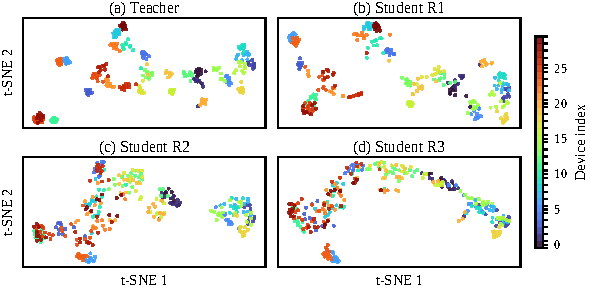
\includegraphics[width=0.95\linewidth]{figures/feature_visualization.pdf}
    \caption{Embedding space visualization and iterative distillation trajectory for ResNet across three compression rounds.}
    \label{fig:iterative}
\end{figure}

\begin{table}[t]
\caption{Per-layer PCA effective dimensions across iterative distillation rounds on ResNet.}
\label{tab:iterative_trace}
\centering
\footnotesize
\setlength{\tabcolsep}{5.5pt} % 优化间距，使多行表头排版更紧凑
\begin{tabular}{l|c|r|c|c|c}
\toprule
\textbf{Round} & \textbf{Channel Config} & \textbf{Params} & \textbf{LOS} & \textbf{NLOS} & \textbf{Walk} \\
& $[c_1, c_2, c_3, c_4, c_5]$ & & \textbf{-A} & \textbf{-D} & \textbf{-F} \\
\midrule
Teacher & [32, 32, 32, 64, 64] & 203,264 & 99.70 & 100.00 & 98.90 \\
Round 1 & [10, 12, 13, 19, 7]  & 13,784  & 99.80 & 99.40  & 99.40 \\
Round 2 & [8, 9, 4, 4, 4]       & 3,024   & 96.95 & 97.05  & 90.85 \\
Round 3 & [5, 6, 3, 2, 2]       & 1,364   & 96.00 & 92.70  & 96.85 \\
\bottomrule
\end{tabular}
\vspace{2pt}
\begin{tablenotes}
\footnotesize
\item[*] Note: LOS-A, NLOS-D, and Walk-F represent static line-of-sight, complex non-line-of-sight, and dynamic walking environments, respectively.
\end{tablenotes}
\end{table}

\subsection{Inference Latency on Edge Platforms}

To evaluate the real-time capability of the PCA-derived student networks, we measure inference latency, decomposing end-to-end latency into feature extraction and classification.
Results are reported in the rightmost columns of Table~\ref{tab:final_merged_complete}.

On the Jetson Nano, the ResNet18 teacher backbone requires 4.45~ms for feature extraction and 33.36~ms end-to-end (30~FPS), making it unsuitable for real-time per-packet authentication.
In contrast, all student backbones complete feature extraction in under 1.2~ms, with end-to-end latency ranging from 0.69~ms (DenseNet) to 1.60~ms (ResNet18), corresponding to 625--990~FPS on the same constrained hardware---a throughput that exceeds typical LoRa packet rates by a wide margin.

On the RTX~4090, the student backbones execute feature extraction within 16.7--49.7~$\mu$s per inference.
With PCA-accelerated classification, end-to-end throughput reaches 10,800--17,000~FPS across all student networks.
These results confirm that the proposed automated pipeline produces models that are not only parameter- and storage-efficient, but also latency-optimal for real-time edge RFFI deployment across heterogeneous hardware platforms.


\section{Conclusion}
\label{sec:conclusion}
This paper presents an automated lightweight RFFI pipeline that integrates PCA-driven channel analysis, structural pruning with random reinitialization, and self-distillation via PCA-aligned KL divergence.
By deriving per-layer channel budgets from the PCA energy spectrum of trained networks, the pipeline eliminates manual architecture design and replaces heuristic width multipliers with a data-driven criterion.
Self-distillation enables randomly-initialized compact networks to recover teacher-level discriminability, and we demonstrate that distillation additionally serves as a representation purification mechanism: students of undertrained teachers consistently outperform their teachers.
An iterative extension provides accuracy-bounded progressive compression, automatically pushing the model toward the practical channel-level compression limit.
Experiments across four diverse architectures on a real-world LoRa dataset demonstrate 14--834$\times$ parameter compression with minimal accuracy degradation, and edge deployment on an NVIDIA Jetson Nano achieves over 600~FPS inference throughput.
This work provides a practical, fully automated path toward deploying secure, low-latency RFFI systems on resource-constrained edge platforms without sacrificing performance.


\bibliographystyle{IEEEtran}
\bibliography{references}
\end{document}
